\chapter{Introduction and Problem Statement}

\section{Introduction}
Every academic year, thousands of students from across India relocate to Uttarakhand for higher education. Educational hubs like Dehradun, Roorkee, and Rishikesh host prominent institutions including Graphic Era Hill University (GEHU), Graphic Era University (GEU), UPES, DIT University, Doon University, and IIT Roorkee. For an outstation student moving into these cities for the first time, two immediate practical challenges arise within their first week: finding safe, budget-friendly accommodation (such as a Paying Guest accommodation, student hostel, or shared flat), and acquiring basic daily living essentials—such as a study desk, room cooler, mattress, reference textbooks, or a used two-wheeler—without spending unnecessary money.

Dehradun alone accommodates tens of thousands of outstation students across major campus neighborhoods like Clement Town, Premnagar, Rajpur Road, Ballupur, and Sahastradhara Road. Consequently, the local demand for student housing and affordable second-hand items has grown steadily.

Despite this sustained demand, the local rental and second-hand market in Uttarakhand remains unorganized and frustrating for students. Incoming students often depend on informal local brokers who charge high non-refundable commissions (frequently equal to a full month's rent) simply for sharing contact numbers. Many listings feature misleading photos, unverified amenities, or vague rules regarding security deposit refunds. At the same time, the local market for second-hand student goods is split between cluttered WhatsApp/Telegram groups and general classifieds like OLX, where student listings get buried under dealer ads, spam, and unverified accounts.

To address these everyday challenges, this project presents \textbf{StayMart}—a unified student accommodation discovery and campus re-commerce marketplace web application designed specifically for Uttarakhand. StayMart combines a Java 17 / Spring Boot 3.3 REST backend, a normalized MySQL 8.0 database, an asynchronous Python 3.11 / Flask machine learning microservice for content-based recommendations, and a clean, responsive frontend inspired by established classified platforms like OLX and Amazon.

\section{Motivation}
The driving motivation behind StayMart arises from direct observations and real pain points experienced by university students living around Uttarakhand campus corridors:

\begin{enumerate}
    \item \textbf{High Brokerage Overhead and Financial Drain:} Local property brokers typically charge incoming students between 50\% and 100\% of one month's rent upfront simply for providing a caretaker's phone number. For students managing tight monthly allowances or education loans, paying ₹5,000 to ₹10,000 in non-refundable broker fees creates an immediate financial burden.
    \item \textbf{Misleading Listings and Neighborhood Geography:} Outstation students arriving from other states lack familiarity with Dehradun localities such as Clement Town, Subhash Nagar, Premnagar, and Rajpur Road. Unregulated landlords frequently share misleading photos, conceal room sizes, or fail to mention lack of water storage or power backup during heavy mountain monsoons.
    \item \textbf{Campus Re-Commerce Waste and Lost Savings:} Graduating seniors frequently abandon or sell functional room coolers, study desks, reference textbooks, bicycles, and lab equipment to scrap dealers for nominal sums. Simultaneously, incoming juniors arrive and purchase the exact same items brand new at full retail prices.
    \item \textbf{Shortcomings of Existing Commercial Platforms:} Mainstream platforms fail to address these student-specific needs. Airbnb targets tourists with expensive daily rates; OLX has no room-level vacancy tracking or campus moderation; and platforms like 99acres and MagicBricks are dominated by commercial property brokers.
    \item \textbf{Lack of Contextual Recommendations:} General classifieds display chronological feeds without student-specific filtering. A student searching for a girls' PG near Graphic Era is often shown commercial office spaces or boys' dormitories across distant towns, leading to tedious manual filtering.
\end{enumerate}

\section{Problem Statement}
The practical problem addressed in this project is defined as follows:

\begin{quote}
\textit{``To design and implement a practical, full-stack student accommodation and campus re-commerce marketplace web platform for Uttarakhand university corridors, connecting students directly with verified property owners and student sellers with zero brokerage, room-level availability tracking, direct peer messaging, and content-based recommendations.''}
\end{quote}

The core design challenges addressed include:
\begin{itemize}
    \item \textbf{Dual-Entity Domain Modeling:} Structuring both accommodation entities (room types, meal plans, curfew rules, deposit terms, and amenities) and marketplace products (item condition, category, sell vs. rent workflows) within a coherent database schema.
    \item \textbf{Transactional Consistency in Bookings:} Preventing double-booking of shared room beds and ensuring inventory locks on single-quantity second-hand items.
    \item \textbf{Cold-Start Recommendation Dynamics:} Ensuring newly registered students receive useful, locality-sensitive listings before accumulating extensive browsing history.
    \item \textbf{Clean, Responsive Classifieds UI:} Building a lightweight, intuitive classifieds interface modeled after OLX and Amazon, functioning smoothly across smartphones and laptops without frontend build overhead.
\end{itemize}

\section{Objectives and Project Scope}

\subsection{Primary Objectives}
The specific engineering objectives established for StayMart are:
\begin{enumerate}
    \item \textbf{Architectural Decoupling:} Implement a modular multi-tier architecture separating the Presentation Layer (Vanilla HTML5/CSS3/JavaScript), Core Application Layer (Spring Boot 3.3 REST API on Java 17 LTS), Persistence Layer (MySQL 8.0 InnoDB), and Analytical Intelligence Layer (Flask ML Microservice).
    \item \textbf{Comprehensive Role-Based Security:} Implement stateless authentication using JSON Web Tokens (JWT) signed via HMAC-SHA256, enforcing role-based access control for public visitors, registered students, property caretakers, and platform administrators.
    \item \textbf{Content-Based Recommendation Engine:} Build an automated recommendation service utilizing Term Frequency-Inverse Document Frequency (TF-IDF) vectorization and Cosine Similarity matrices to match listings with student preferences, supported by database fallbacks.
    \item \textbf{Moderation and Listing Verification:} Provide an administrative moderation console enabling platform administrators to review, approve, or reject student and caretaker listings before public display.
    \item \textbf{Direct Peer-to-Peer Messaging:} Provide an internal messaging system allowing students, caretakers, and sellers to discuss room terms and inspect items directly.
    \item \textbf{Production Cloud Readiness:} Provide a containerized multi-tier setup and zero-cost cloud deployment strategy (Vercel static hosting, Render backend containers, and free managed MySQL).
\end{enumerate}

\subsection{Project Scope and Regional Focus}
The geographic and functional boundaries of this project include:
\begin{itemize}
    \item \textbf{Geographic Coverage:} Hyperlocal coverage of student corridors in Uttarakhand: Dehradun (Clement Town near Graphic Era, Premnagar near UPES, Rajpur Road near DIT, Ballupur, Subhash Nagar, Patel Nagar, Sahastradhara Road), Rishikesh (Tapovan), Haridwar, Mussoorie, and Roorkee (Civil Lines near IIT).
    \item \textbf{Target Demographics:} University students, faculty, competitive exam aspirants, and local residential property caretakers.
    \item \textbf{Marketplace Offerings:} Six accommodation classifications (PG, Hostel, Flat, Room, Hotel, Dormitory) and ten consumer re-commerce categories (Electronics, Mobile Phones, Furniture, Books \& Stationery, Home Appliances, Vehicles, Sports \& Fitness, Home \& Kitchen, Fashion, Others).
\end{itemize}

\section{Proposed Framework and Value Proposition}
StayMart provides three key practical advantages over informal methods:

\begin{figure}[htbp]
    \centering
    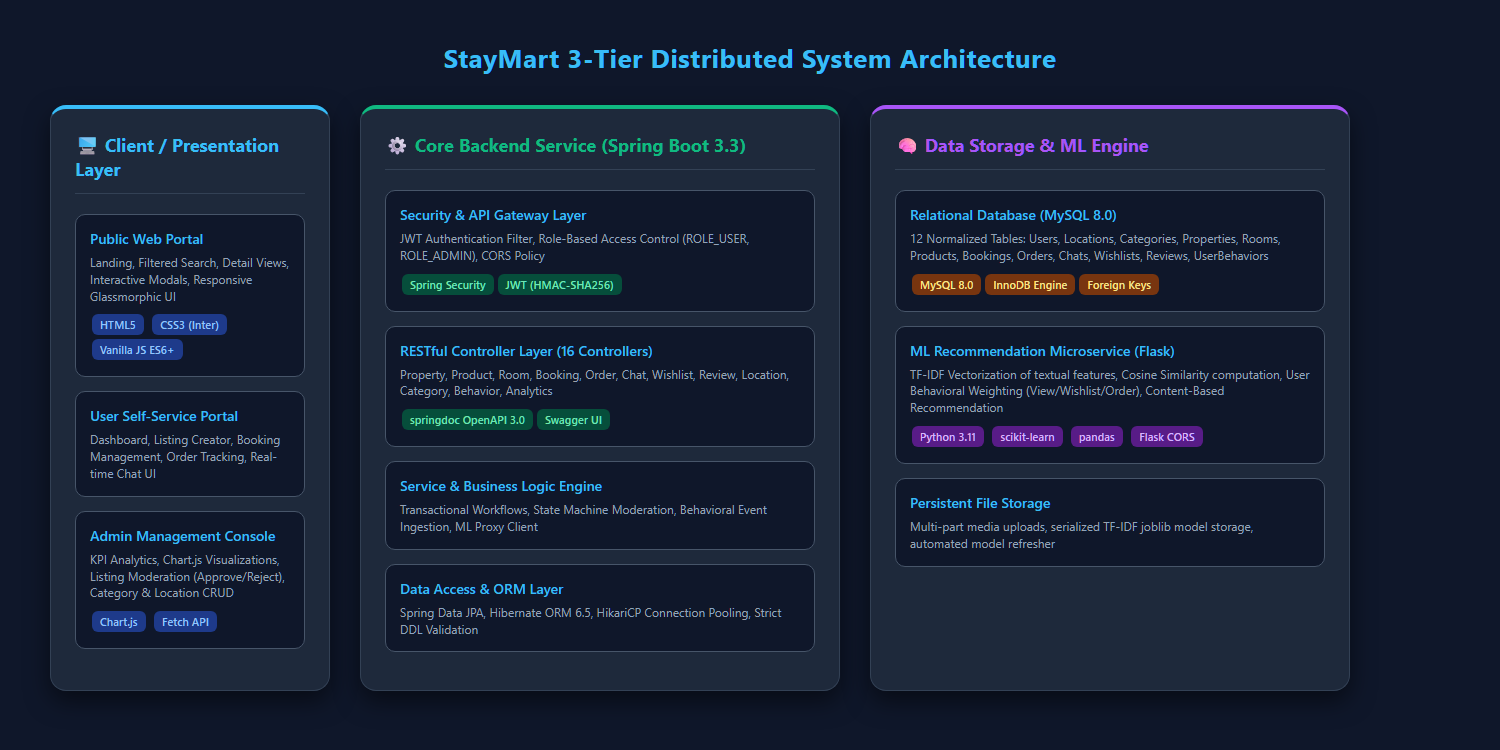
\includegraphics[width=0.95\textwidth]{diagrams/arch_diagram.png}
    \caption{High-Level Distributed Framework of the StayMart Platform}
    \label{fig:framework_overview}
\end{figure}

\begin{enumerate}
    \item \textbf{Zero-Brokerage Direct Connection:} Connects students directly with verified property caretakers and student sellers without middleman commissions, keeping off-campus housing affordable.
    \item \textbf{Verified Photographic Asset Standard:} Listings emphasize authentic photographs of rooms, study desks, and equipment taken by students and caretakers rather than generic stock imagery.
    \item \textbf{Contextual Recommendations:} Combines text similarity matching with user interactions (views, wishlists, and inquiries) to highlight relevant listings near the student's campus.
\end{enumerate}

\section{Organization of the Project Report}
The project report is organized into the following chapters:
\begin{itemize}
    \item \textbf{Chapter 2 (Literature Review):} Evaluates existing classified platforms (OLX, Airbnb, MagicBricks), recommendation algorithms (Content-Based vs. Collaborative Filtering), microservice architecture patterns, and identifies practical gaps in current tools.
    \item \textbf{Chapter 3 (System Requirements and Architecture):} Outlines the Software Requirements Specification (SRS), functional and non-functional requirements, UML diagrams, and Data Flow Diagrams (DFD Level 0, 1, and 2).
    \item \textbf{Chapter 4 (Database Design and Relational Modeling):} Explains the MySQL relational schema, Entity-Relationship (ER) diagrams, normalization analysis (1NF through BCNF), and data dictionaries for all 12 tables.
    \item \textbf{Chapter 5 (Backend and ML Microservice Implementation):} Details the Spring Boot 3.3 (Java 17 LTS) backend, stateless JWT security, the Python TF-IDF recommendation pipeline, and the resilient database fallback mechanism.
    \item \textbf{Chapter 6 (Frontend UI/UX Design System):} Presents the OLX and Amazon-inspired responsive design system, design tokens, and modular client-side JavaScript architecture.
    \item \textbf{Chapter 7 (Verification, Testing and Visual Walkthrough):} Documents testing methodologies, unit/integration test results, automated mobile viewport tests, and an illustrated system walkthrough.
    \item \textbf{Chapter 8 (Deployment, Cloud Hosting and Startup Guide):} Details free-tier cloud deployment on Vercel, Render, and TiDB Serverless, along with a local development runbook.
    \item \textbf{Chapter 9 (Conclusion and Future Scope):} Summarizes project contributions, reflections, limitations, and the future development roadmap.
    \item \textbf{Appendices \& References:} Provide the REST API catalog, data schemas, and academic citations.
\end{itemize}
